\documentclass[journal,12pt,onecolumn]{IEEEtran}
\usepackage{cite}
 \usepackage{caption}
\usepackage{graphicx}
\usepackage{amsmath,amssymb,amsfonts,amsthm}
\usepackage{algorithmic}
\usepackage{graphicx}
\usepackage{textcomp}
\usepackage{xcolor}
\usepackage{txfonts}
\usepackage{listings}
\usepackage{enumitem}
\usepackage{mathtools}
\usepackage{gensymb}
\usepackage{comment}
\usepackage[breaklinks=true]{hyperref}
\usepackage{tkz-euclide} 
\usepackage{listings}
\usepackage{gvv}
%\def\inputGnumericTable{}                                 
\usepackage[latin1]{inputenc} 
\usetikzlibrary{arrows.meta, positioning}
\usepackage{xparse}
\usepackage{color}                                            
\usepackage{array}                                            
\usepackage{longtable}                                       
\usepackage{calc}                                             
\usepackage{multirow}
\usepackage{multicol}
\usepackage{hhline}                                           
\usepackage{ifthen}                                           
\usepackage{lscape}
\usepackage{tabularx}
\usepackage{array}
\usepackage{float}

\usepackage{float}
%\newcommand{\define}{\stackrel{\triangle}{=}}
\theoremstyle{remark}
\usepackage{circuitikz}
\captionsetup{justification=centering}
\usepackage{tikz}

\title{Matrices in Geometry 1.9.24}
\author{EE25BTECH11035 - Kushal B N}
\begin{document}
\vspace{3cm}
\maketitle
{\let\newpage\relax\maketitle}
\textbf{Question: }
The x-coordinate of a point $\vec{P}$ is twice is y-coordinate. If $\vec{P}$ is equidistant from the points $\vec{Q}$$\brak{2,-5}$ and $\vec{R}$$\brak{-3,6}$, find the coordiantes of $\vec{P}$.\\

\textbf{Given: } \\
$\vec{P}$$\myvec{2k\\k}$, $\vec{Q}\myvec{2\\-5}$, $\vec{R}\myvec{-3\\6}$.\\
Distances $PQ$ = $PR$

So their norms must be equal and also the square of their norms.
\begin{equation}
	{\norm{\vec{Q}-\vec{P}}}^{2} = {\norm{\vec{R}-\vec{P}}}^{2}
\end{equation}

\begin{equation}
    {\norm{\vec{P}}}^2 - 2\vec{P}^{\top}\vec{Q} + {\norm{\vec{Q}}}^2 = {\norm{\vec{P}}}^2 - 2\vec{P}^{\top}\vec{R} + {\norm{\vec{R}}}^2
\end{equation}

\begin{equation}
    \implies \frac{{\norm{\vec{Q}}}^2 - {\norm{\vec{R}}}^2}{2} = \vec{P}^{\top}\brak{\vec{Q}-\vec{R}}
\end{equation}

\begin{equation}
    {\norm{\vec{Q}}}^2 = \myvec{2&-5}\myvec{2\\-5} = 4+25 = 29
\end{equation}

\begin{equation}
    {\norm{\vec{R}}}^2 = \myvec{-3&6}\myvec{-3\\6} = 9+36 = 45
\end{equation}

\begin{equation}
    \vec{Q} - \vec{R} = \myvec{5\\-11}
\end{equation}

\begin{equation}
    \implies -8 = \myvec{2k&k}\myvec{5\\-11}
\end{equation}

\begin{equation}
    -8 = 10k - 11k = -k
\end{equation}

\begin{equation}
    \implies \fbox{k = 8}
\end{equation}
   

\bigskip

\textbf{Final Answer: }
The coordinates of point $\vec{P} = \myvec{16\\8}$.

\begin{figure}
    \centering
    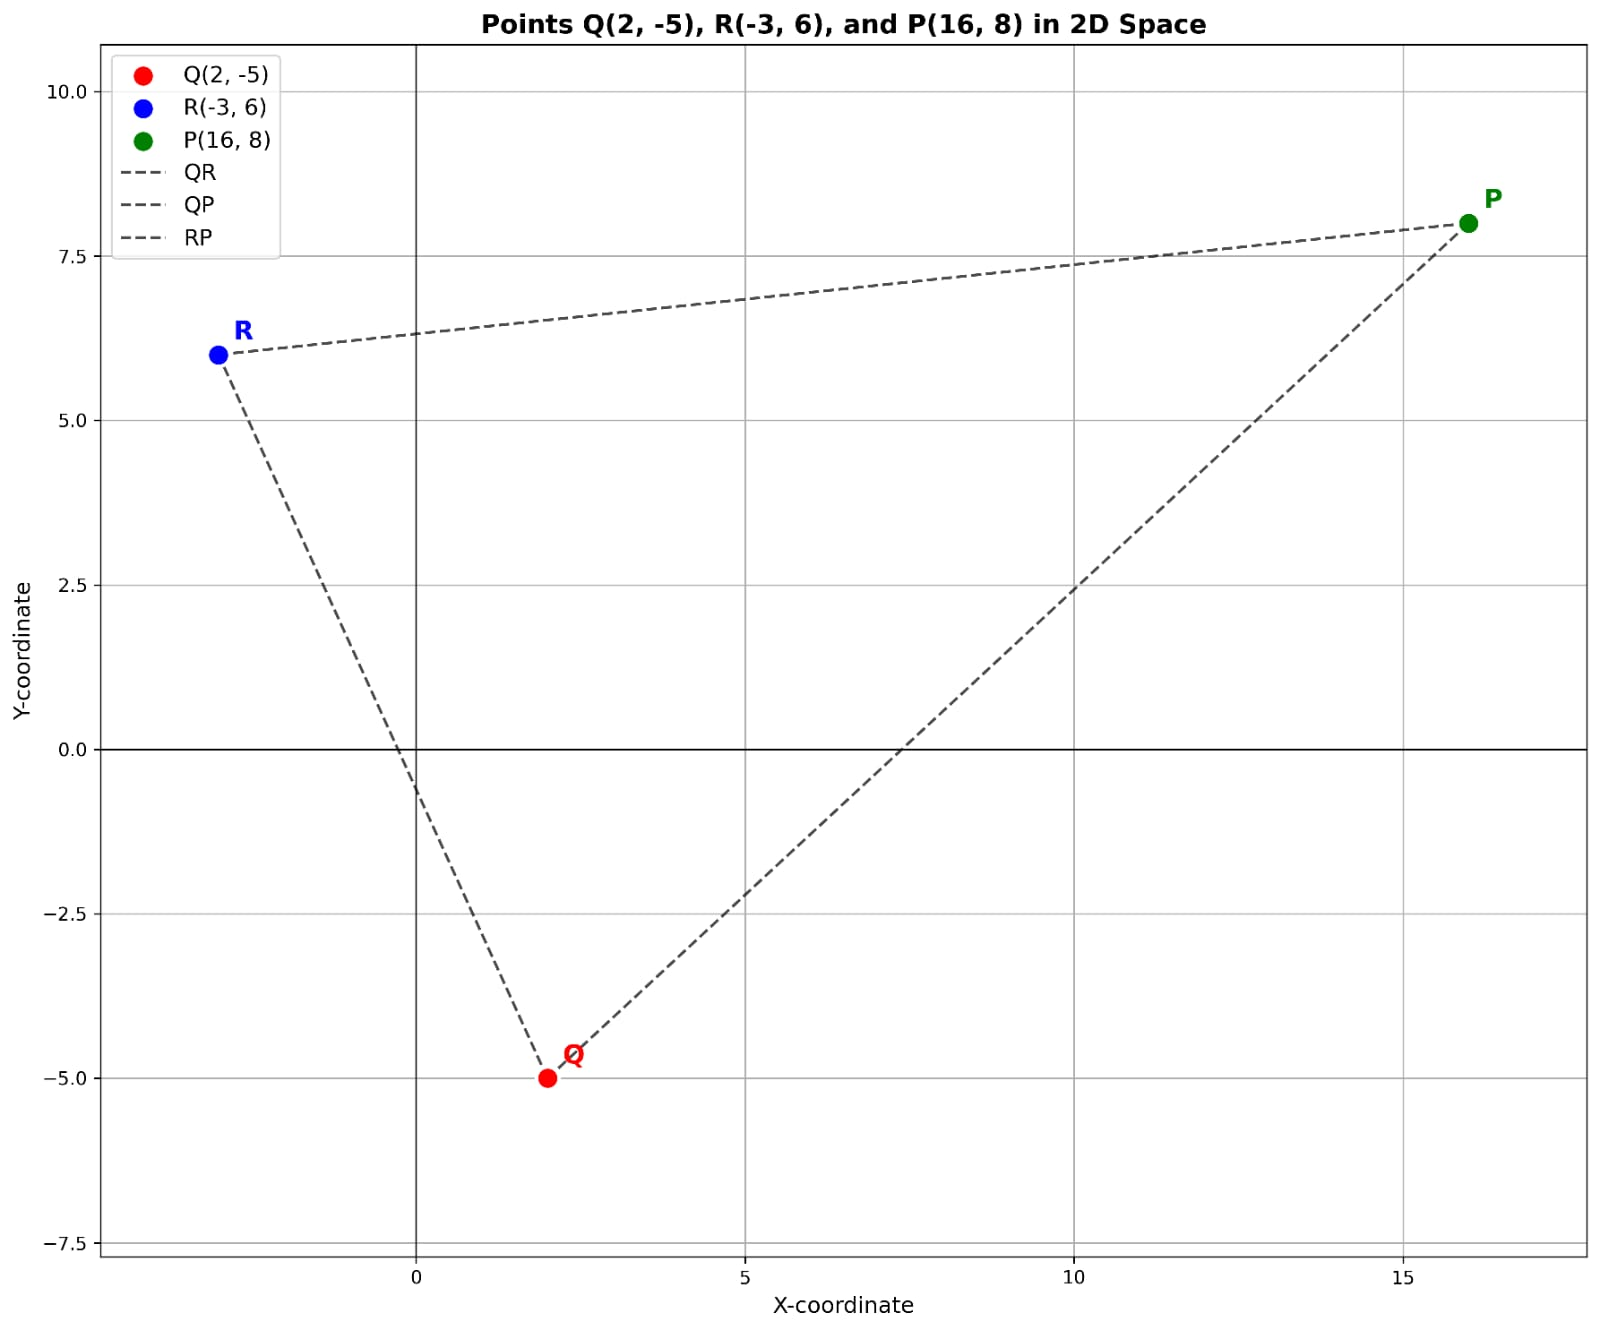
\includegraphics[width=1\columnwidth]{figs/1.jpg}
    \caption{Plot of the three points in 2-D Space}
    \label{fig:placeholder}
\end{figure}


\end{document}
